\documentclass{article}

\PassOptionsToPackage{numbers,compress}{natbib}
\usepackage[preprint]{neurips_2025}

\usepackage[utf8]{inputenc}
\usepackage[T1]{fontenc}
\usepackage{hyperref}
\usepackage{url}
\usepackage{booktabs}
\usepackage{amsfonts}
\usepackage{amsmath}
\usepackage{amssymb}
\usepackage{mathtools}
\usepackage{microtype}
\usepackage{xcolor}
\usepackage{tabularx}
\usepackage{array}
\usepackage{float}
\usepackage{graphicx}
\usepackage{rotating}
\hypersetup{hypertexnames=false,hidelinks}

\newcolumntype{Y}{>{\raggedright\arraybackslash}X}
\newcommand{\1}{\mathbf{1}}
\newcommand{\Bpos}{\mathcal B_x^+}
\newcommand{\sg}{\operatorname{sg}}
\DeclareMathOperator{\clip}{clip}

\title{ModeBench: Executable Outcome Discovery\\
for Maximum-Entropy Reasoning}

\author{Anonymous Authors}

\begin{document}

\maketitle

\begin{abstract}
Reinforcement learning with binary verifiers can make a reasoning policy more
accurate while concentrating it on one successful output. Studying this
failure requires more than \texttt{pass@1}: the task must admit multiple
solutions, validate them without heuristic text matching, and decide when two
successful responses are genuinely different. We introduce \textsc{ModeBench},
a suite and execution contract for that setting. Its four synthetic domains
cover constraint assignments, arithmetic expression trees, Python functions,
and executable algebra action menus. In every domain, correctness and mode
identity are derived from the same executed object. The Python domain runs a
syntax-restricted function in an isolated external interpreter and contains
16--3,600 exact behavior modes per instance.

We pair the benchmark with online verified MaxEnt. For each prompt, training
maintains a bank containing only outcomes generated by the policy and accepted
by the task validator. An open-set predictive distribution over that bank plus
one structural unseen bucket supplies a centered surprisal advantage, a
one-time bonus rewards new discoveries, and a global round-robin scheduler
replays exactly one previously discovered verified bank per optimizer update
under split verified-mass and known-mode-balance terms. All three coefficients
are self-warmup and carry no projection, so a fixed-budget matched study is a
direct stress test of both collapse and runaway pressure.

The confirmatory campaign is 54 registered runs and is still executing, so we
report an explicitly interim, fixed-checkpoint snapshot and no terminal claim.
At the latest checkpoint that all three seeds of both arms have landed,
verified MaxEnt raises \texttt{pass@8} over matched Dr.GRPO from .372 to .968
on graph coloring (pass 10), .608 to .665 on Countdown (pass 5), .172 to .740
on Python factors (pass 6), and .266 to .663 on MathIR action menus (pass 5),
with distinct correct modes rising from .393 to 2.344, .650 to 1.674, .172 to
.956, and .266 to .682. On held-out MATH-500 after training on frozen
MATH12K-384, the two arms remain within .01 of each other on greedy
\texttt{pass@1} at pass 2. All four prospectively frozen interpretation gates
are \texttt{pending}; none may be read as a result. The main contribution is
the validator-bound experimental object: it separates semantic discovery from
surface variation and makes long-horizon mode collapse measurable.
\end{abstract}

\section{Introduction}
\label{sec:introduction}

Verifier-based reinforcement learning is indifferent among correct responses
when every one receives reward one. That symmetry does not imply that a learned
policy remains broad. Group-relative updates can repeatedly reinforce the
successful output that happened to be sampled, after which future groups see
less of the alternatives. A policy may therefore improve per-sample
correctness while becoming worse at test-time search, self-consistency, or
future learning from rare solutions
\citep{wang2023selfconsistency,song2025outcome,li2025divergence}.

Maximum-entropy reinforcement learning is a natural response
\citep{ziebart2008maximum,haarnoja18b,levine2018control}, but language-model
entropy is not solution entropy. A free-form response can vary in wording,
derivation length, formatting, and termination while expressing the same
answer. Our preliminary program made this distinction concrete. Direct
sequence entropy could be spent on longer responses and avoiding EOS;
candidate-level projections introduced length-dependent biases or optimized a
detached improvement target rather than policy entropy; and sampled
surprisal lost its actuator as groups concentrated. Outcome-level shaping was
denser, but current-group collision penalties could not distinguish tail
singletons, empirical centering could erase a shared novelty signal, and
unrestricted novelty could reward distinct errors. Latent option objectives
faced the complementary problem: correct answer repetitions were too sparse
to estimate binding cleanly.

Those negative results point to a stricter experimental object. An outcome
should enter the diversity objective only if:

\begin{enumerate}
  \item the current policy actually generated it;
  \item an executable task validator accepted that exact generation;
  \item the canonical key is derived from the same execution that established
  correctness; and
  \item the diversity signal is applied outside the empirical centering that
  can erase it.
\end{enumerate}

\textsc{ModeBench} implements that object. Graph coloring validates a complete
assignment against every edge. Countdown parses an arithmetic AST, enforces
exact operand use, and executes it against the target. Python factor functions
are called by an isolated external interpreter on a frozen prompt-local test
suite; the vector returned by those calls is the mode. MathIR action menus
execute a bounded sequence of equation transformations under exact rational
arithmetic; the normalized state trajectory is the mode. The domains
deliberately span a direct combinatorial object, an expression, program
behavior, and an algebraic procedure.

Our training method builds a prompt-local verified bank online. It neither
starts from a gold answer catalogue nor divides training into discovery and
exploitation phases. Every group can add validator-positive outcomes and learn
from their frequencies. Because a discovered outcome must otherwise wait for
its own prompt to reappear, a global round-robin scheduler replays exactly one
previously discovered verified bank on every optimizer update. Because a fixed
coefficient bound can become the active constraint precisely when collapse is
strongest, every controller is projection-free and referenced only to its own
warmup statistic.

Our contributions are:

\begin{itemize}
  \item \textsc{ModeBench}, a four-domain benchmark in which correctness and
  semantic identity share one executable validation path;
  \item an online growing-support objective that rewards rare and newly
  discovered verified modes without a gold support catalogue, and that makes
  discoveries act promptly through a globally scheduled verified replay;
  \item three projection-free, self-referenced coefficient controllers with
  passive, method-neutral discovery telemetry in the matched control;
  \item a separated-support entropy-gated singleton actuator whose proposals
  may reach the replay layer but never the on-policy advantage; and
  \item a prospectively frozen 54-run, 12-pass campaign with fixed reporting
  checkpoints, four registered interpretation gates, and a fail-closed audit
  chain, reported here as an explicitly interim snapshot.
\end{itemize}

\section{Related Work}
\label{sec:related}

\paragraph{Verifier-based reasoning RL.}
Group-relative optimization is widely used to train reasoning models from
outcome rewards \citep{shao2024deepseekmath,guo2025deepseekr1,
liu2025understanding}. Sampling several responses can improve aggregate
success, but it also exposes a distinction between per-draw accuracy and
support coverage. Countdown has served as a compact environment for learning
search from verifiers \citep{gandhi2024stream,tinyzero2025}. We focus on tasks
small enough to audit mode identity exactly.

\paragraph{Diversity-aware policy optimization.}
Prior approaches reward rare historical answers, penalize repeated outcomes,
encourage token-level differences among positive responses, change the
group-level pass@\(\!k\) objective, or preserve mass relative to a reference
policy \citep{song2025outcome,divpo2025,chen2025passktraining,
li2025divergence}. These mechanisms act on complementary objects. Our
distinction is the admission boundary: a novelty key exists only after the
same generated object passes an executable validator.

\paragraph{Maximum-entropy control.}
Entropy-regularized control augments expected reward with policy entropy and
admits both regularized-MDP and probabilistic-inference views
\citep{ziebart2008maximum,geist2019regmdp,levine2018control}. Soft Actor-Critic
adapts the entropy coefficient with a dual update
\citep{haarnoja18b,haarnoja2018algorithms}. We borrow the automatic
coefficient principle, not SAC's critic, replay buffer, or off-policy
objective. Our sensor is an empirical distribution over verified outcomes
generated by an on-policy language model, and our controllers are referenced
to their own warmup means rather than to an externally supplied target.

\paragraph{Executable and grammar-constrained outputs.}
Formal grammars can prevent invalid generations
\citep{geng2023grammar}. \textsc{ModeBench} uses a different boundary:
generation may remain free-form for graph coloring and Countdown, but
admission is fail-closed. The Python domain additionally restricts its
one-line language before an external call, and MathIR restricts its command
alphabet before execution. In all cases, execution determines both reward and
identity.

\section{ModeBench}
\label{sec:modebench}

\subsection{Benchmark contract}

For prompt \(x\), response \(y\), and reference specification \(s_x\), a task
provides one function
\[
V(y,s_x)\in\{\bot\}\cup\mathcal C_x .
\]
The value \(\bot\) means invalid or incorrect. Otherwise \(V\) returns a
canonical key \(c\in\mathcal C_x\). Reward and identity are inseparable:
\[
r(x,y)=\1[V(y,s_x)\neq\bot],
\qquad
c(x,y)=V(y,s_x)\quad\text{when }r=1.
\]
A benchmark is mode-verifiable only if two properties hold. First, the
validator checks the object actually generated, rather than a model-supplied
claim about it. Second, formatting aliases do not create new keys, while
different executed outcomes do.

\begin{table}[H]
  \centering
  \small
  \setlength{\tabcolsep}{4pt}
  \begin{tabularx}{\linewidth}{@{}lYYY@{}}
    \toprule
    \textbf{Domain} & \textbf{Generated object} &
    \textbf{Executable check} & \textbf{Mode key} \\
    \midrule
    Graph coloring &
    Missing colors or a full assignment &
    Materialize the assignment; check fixed colors and every edge &
    Complete color vector \\
    Countdown &
    Arithmetic expression &
    Parse AST; check exact multiset of operands; evaluate exactly &
    Normalized executed AST \\
    Python factors &
    One-line \texttt{lambda n: EXPR} &
    Call in an isolated Python worker on every frozen input; check proper
    divisibility &
    Returned integer vector \\
    MathIR action menu &
    Bounded sequence of menu actions &
    Apply each command to both sides; normalize exactly after every step &
    Normalized equation-state trajectory \\
    \bottomrule
  \end{tabularx}
  \caption{\textbf{The four ModeBench environments.} Correctness and mode
  identity come from the same executed object.}
  \label{tab:tasks}
\end{table}

\subsection{Graph coloring}

Each instance describes a graph, a partial three-color assignment, and several
hidden vertices. The response supplies the missing digits or the complete
assignment. The validator fixes shown colors, reconstructs the full vector,
and rejects any monochromatic edge. The canonical key is that full vector, so
spacing and answer formatting are aliases but different valid completions are
different modes. The current train/evaluation split contains 192/96 prompts.

\subsection{Countdown}

Each instance supplies three distinct integers and a target. A response uses
each input exactly once with \(+,-,\times,\div\) and parentheses. The validator
parses only this arithmetic subset, evaluates with exact rational arithmetic,
and requires the target. Commutative children are sorted in the canonical AST,
so \(2+3\times4\) and \(4\times3+2\) share a key, while genuinely different
expression trees remain distinct. The split contains 384/128 prompts.

\subsection{Python factor functions}
\label{sec:python-task}

The third environment tests program behavior rather than source appearance.
Each prompt lists four composite integers and requests a pure function with
the exact signature \texttt{lambda n: EXPR}. For every frozen tool call, the
returned value \(d\) must satisfy
\[
1<d<n,\qquad n\bmod d=0.
\]
The accepted syntax contains integer literals, the variable \(n\), bounded
arithmetic, comparisons, Boolean operators, and conditional expressions.
Calls, imports, attributes, containers, comprehensions, subscripts, loops,
and other names are rejected before execution.

After syntax validation, a persistent isolated Python worker calls the
function. The worker returns either failure or the complete output vector;
the parent process never evaluates model code. If the inputs are
\((n_1,\ldots,n_m)\) and \(D(n)\) is the set of nontrivial proper divisors,
then the exact number of semantic modes is
\[
M(x)=\prod_{j=1}^{m}|D(n_j)|.
\]
The released deterministic materialization has 384 training and 128
evaluation prompts, disjoint input tuples, and 16--3,600 modes per prompt.
For every row, the generator constructs two different functions and requires
the external worker to certify two different behavior keys.

\subsection{MathIR action menus}
\label{sec:mathir-task}

The fourth environment keeps the executable contract while moving closer to
ordinary algebra. Each prompt shows a linear equation and a finite lettered
menu of at most eight equation transformations. A response emits a bounded
sequence of menu actions rather than prose or a final numeric answer. The
interpreter applies each selected command to both sides of the current
equation and renormalizes with exact rational arithmetic after every step;
there is no parser for LaTeX, natural-language derivations, or a
model-declared answer. Programs are limited to four steps.

The canonical key is the normalized state trajectory produced by that
successful execution, so two different routes to the same solved equation are
different modes and two spellings of the same route are the same mode. The
deterministic materialization \texttt{mathir\_action\_menu\_v1} uses seed
5900, contains 384 training and 128 evaluation prompts over four equation
families, and has exactly five exhaustively enumerated modes per prompt. The
enumerated support is used by evaluation only; the training bank starts
empty and no gold catalogue is supplied to the policy.

\section{Online Verified Maximum Entropy}
\label{sec:method}

\subsection{Growing verified support}

For each prompt \(x\), the learner maintains a bank
\(\Bpos\) of canonical keys that the current policy has generated and the
validator has accepted. The bank starts empty. A reference specification may
define the task constraints, but no gold answer catalogue initializes the
bank.

For each generated response, the learner decodes the exact training
trajectory and independently calls \(V\). Admission is fail-closed at the
intersection of executable canonical validation and positive rollout reward;
a disagreement is excluded from both passive tracking and the active bank and
is recorded in telemetry. All candidates in a group are scored against one
immutable pre-group snapshot, and new keys are committed only after the whole
group is scored, so novelty is invariant to row order. Counts, bank state,
scheduler cursor, and all controller states are stored in optimizer-resumable
checkpoints and must all be present on resume.

\subsection{Open-set semantic advantage and discovery credit}

Consider a group of \(G=16\) responses for prompt \(x\). Let \(c_x(a)\)
collect the historical bank count of verified key \(a\) together with the
leave-one-out multiplicity of \(a\) among the other verified responses in the
current group, let \(K_x\) be the number of explicitly counted keys, and let
\(\lambda=1\) be a pseudocount. The predictive distribution always carries one
structural unseen bucket \(\varnothing\):
\[
q(a)=\frac{c_x(a)+\lambda}{\sum_b c_x(b)+\lambda(K_x+1)},
\qquad
q(\varnothing)=\frac{\lambda}{\sum_b c_x(b)+\lambda(K_x+1)} .
\]
With surprisal clip \(S=5\),
\[
h_i=\min\{-\log q(a_i),S\},
\qquad
\overline h=\sum_{a\in\mathcal K_x\cup\{\varnothing\}}
q(a)\min\{-\log q(a),S\},
\qquad
A_i^{\mathrm{sem}}=\beta_t\,\frac{h_i-\overline h}{S}.
\]
The advantage is centered under the detached predictive distribution, not by
the empirical mean of the sampled group, so it can remain nonzero when the
current correct samples all share one mode but the bank records alternatives.
The unseen bucket keeps the objective open: it never asserts that the
discovered support is complete.

Let \(\mathcal N_x\) be current verified keys absent from the pre-group bank.
The discovery advantage is
\[
A_i^{\mathrm{new}}
=\nu\,\frac{\1[a_i\in\mathcal N_x]}{m_x(a_i)},
\qquad \nu=0.50,
\]
where \(m_x(a_i)\) is the multiplicity of \(a_i\) among current verified
responses. All copies of one newly discovered key share a total credit of
\(\nu\); duplicates and row order cannot multiply discovery reward.

The final actor advantage is
\[
A_i =
\underbrace{r_i-\frac1G\sum_jr_j}_{A_i^{\mathrm{task}}}
+\1[V(y_i,s_x)\neq\bot]
\left(A_i^{\mathrm{sem}}+A_i^{\mathrm{new}}\right).
\]
Wrong, unparseable, and loss-inactive responses receive no canonical
pressure. The task reward entering Dr.GRPO is unchanged, and there is no
second empirical centering after the canonical terms are added. The historical
prompt-local bank-entropy advantage is disabled in every registered arm
(\texttt{bank\_alpha}\(=0\)); the open-set term above is the sole entropy
channel in the actor advantage.

\subsection{Global verified replay}
\label{sec:replay}

A prompt-local bank that is materialized only when its own prompt returns to
the rollout is a slow actuator. With 384 unique training prompts, a singleton
discovered late in one pass can act once and then wait nearly a full pass. The
verified-mass controller then receives sparse observations, the balance
controller stays ineligible until one prompt independently reveals two modes,
and correct executable structure cannot propagate promptly.

After the model creates its first validator-positive bank, every optimizer
update therefore materializes exactly one previously discovered verified bank,
traversed in deterministic round-robin order over prompt hashes with a
checkpointed cursor. A bank contributes at most one stored model-generated
exemplar per observed canonical outcome, up to a fixed replay capacity of 16
outcomes. The scheduled bank receives two independent terms:

\begin{itemize}
  \item \textbf{verified mass}: uniform verified-exemplar likelihood over
  every scheduled bank, including a singleton, with coefficient \(\mu_t\); and
  \item \textbf{known-mode balance}: \(\mathrm{KL}(U_{\mathrm{bank}}\,\|\,
  q_{\mathrm{model}})\) for banks with at least two observed modes, with
  coefficient \(\alpha_t\).
\end{itemize}

With one scheduled bank per update, the replay contribution to the loss is
\(\tfrac{15}{16}\cdot\tfrac1{16}\,(\mu_t L_{\mathrm{mass}}
+\alpha_t L_{\mathrm{balance}})\). Selection sees only the accumulated
verified banks and the fixed one-bank compute budget. It never reads
exhaustive support, a gold mode count, evaluation output, a desired entropy,
or a desired success rate. Before the first verified discovery there is no
eligible bank and therefore no replay gradient.

\subsection{Projection-free self-referenced control}
\label{sec:controllers}

Three coefficients adapt, each from its own sensor and each referenced only to
its own warmup mean over 64 eligible observations with EMA decay \(0.9\). Let
\(\rho\) be the normalized open-set predictive entropy
\(H(q)/\log(K_x+1)\), let \(s\) be the verified-exemplar surprisal, and let
\(h\) be the scheduled bank's normalized entropy. After warmup,
\[
\beta_t=0.10\,\frac{\rho_{\mathrm{ref}}}{\rho_{\mathrm{ema}}},
\qquad
\mu_t=0.10\,\frac{s_{\mathrm{ema}}}{s_{\mathrm{ref}}},
\qquad
\alpha_t=0.10\,\frac{h_{\mathrm{ref}}}{h_{\mathrm{ema}}} .
\]
Falling semantic entropy raises exploration pressure, rising surprisal on
known-correct exemplars raises mass pressure, and falling bank entropy raises
balance pressure. During warmup each coefficient holds its registered
reference dose of \(0.10\). No coefficient has a lower or upper projection, so
sustained collapse can keep increasing pressure and saturation cannot be
mistaken for stability. Singleton banks are skipped by the balance sensor
rather than recorded as zero entropy, which would drive \(\alpha\) upward
before a second outcome exists. Direct token entropy and its controller are
absent from the objective.

\subsection{Why the control also tracks discoveries}

The matched Dr.GRPO arm runs the same validator and maintains the same
prompt-local counts as a passive observer. Its semantic, novelty, mass, and
balance coefficients are exactly zero, so its exploration advantage is
identically zero and cannot enter the loss. This makes cumulative discoveries,
tracked prompts, and mean support comparable without giving the treatment a
private measurement instrument.

\section{The Separated-Support Singleton Actuator}
\label{sec:actuator}

Every mechanism in Section~\ref{sec:method} needs at least one alternative to
act on. When a prompt's bank holds exactly one outcome, the balance term is
ineligible, the open-set advantage has a single explicit bucket, and the
learner can only wait for the policy to rediscover breadth on its own. The
registered treatment adds one support-only escape actuator for exactly that
state.

For the current prompt, a counterfactual proposal is eligible only when all of
the following hold: the bank contains exactly one outcome; the open-set
controller has completed its fixed 64-observation warmup; its current
normalized predictive-entropy EMA is below the run's own warmup reference; and
its unprojected multiplier is therefore greater than one. The proposal starts
from the model's own reward-positive, executable response, applies
domain-specific validator-preserving transformations, and independently
revalidates before and after tokenization. At most one novel outcome may be
admitted per group; a bank with zero or with two or more outcomes is
ineligible.

Two isolation properties make this an actuator rather than a second objective.
First, proposal rows never enter PPO. Second, under the registered separation
contract, proposal-derived outcomes may enter the replay-exemplar layer but
may not enter the historical on-policy count table used by the open-set or
novelty advantages. A proposed outcome therefore remains novel to the
objective until the neutral policy itself produces and validates it, at which
point it receives the ordinary discovery credit, graduates into the on-policy
count table, and its neutral exemplar replaces the proposal-only exemplar.
The singleton condition is an actuator-identifiability test; it is not a claim
that a task has exactly two valid modes.

Because enabling proposals also requires replicated free-form sampling and
local actor weight synchronization, the actuator cannot be evaluated against
the historical treatment alone. The campaign therefore registers a
same-plumbing control that runs the identical objective and execution surface
with proposals and the singleton gate switched off. That control, not the
historical arm, is the causal comparator.

\section{Experimental Design}
\label{sec:experiments}

All runs use Qwen2.5-0.5B-Instruct at a pinned revision, seeds 43, 44, and 45,
group size 16, learning rate \(2\times10^{-7}\), one PPO epoch,
\(\beta_{\mathrm{KL}}=0\), rollout temperature 1, top-\(p=1\), maximum
response length 192, and exactly 12 complete passes through each domain's
fixed training pool. Within a domain, arms share the dataset, source snapshot,
model, optimizer, prompt formatting, rollout count, training budget,
evaluation cadence, evaluation seed, checkpoint cadence, and recovery rules.

\paragraph{Registered surface.}
The confirmatory campaign contains 54 runs across five reporting domains and
four arms, summarized in Table~\ref{tab:campaign}. Two earlier cohorts are
excluded from that denominator by machine-readable invalidation audits rather
than by inspection of their results: one because its runtime forced the
novelty credit to zero before the actuator could fire, and one because its
shared proposal/on-policy bank was rejected by a fail-closed argument
validator before any optimizer step, leaving no training metrics at all.
Their trajectories remain archived as engineering evidence.

\begin{table}[H]
  \centering
  \small
  \setlength{\tabcolsep}{5pt}
  \begin{tabularx}{\linewidth}{@{}lYcc@{}}
    \toprule
    \textbf{Arm} & \textbf{Role} & \textbf{Domains} & \textbf{Runs} \\
    \midrule
    Matched Dr.GRPO & Control with passive verified tracking &
    4 ModeBench \(+\) MATH-500 & \(12+3\) \\
    Verified MaxEnt (global replay) & Method under test &
    4 ModeBench \(+\) MATH-500 & \(12+3\) \\
    Same-plumbing actuator-off & Causal comparator for the actuator &
    4 ModeBench & 12 \\
    Separated-support actuator & Registered repair &
    4 ModeBench & 12 \\
    \bottomrule
  \end{tabularx}
  \caption{\textbf{The 54-run registered campaign.} Each cell is three seeds
  per domain. MATH-500 carries only the two method arms because a
  single-answer task cannot exercise a multi-mode actuator.}
  \label{tab:campaign}
\end{table}

\paragraph{Held-out realism track.}
The fifth reporting domain is an external-validity track, not a fifth
multi-mode environment. Both method arms train on exactly 384 frozen MATH12K
rows and evaluate on all 500 held-out MATH-500 problems, with hash-pinned
train and evaluation materializations and exactly zero normalized problem
overlap. Every verifier-positive completion for a prompt maps to one
prompt-local key, so verified support is structurally at most one: verified
mass may anchor a model-generated correct solution, known-mode balance is
structurally ineligible and must emit zero loss and zero controller
observations, and \texttt{distinct@8} is not reported as reasoning-mode
coverage. Equivalent renderings of one answer cannot masquerade as modes.

\paragraph{Fixed reporting checkpoints.}
The paper surface uses at most ten checkpoints per environment: passes
\(0,1,2,3,4,5,6,8,10,12\) for ModeBench and \(0,2,4,6,8,10,12\) for MATH-500.
Every quarter pass, evaluation records greedy \texttt{pass@1} and four
deterministic temperature-one draws of \(K=8\) responses; the intermediate
records are retained for safety auditing and for the supplemental diagnostic
in Appendix~\ref{app:diagnostic}, but the confirmatory plot, tables, and AUC
use only the registered anchors. We report \texttt{pass@8}, \texttt{mean@8},
\texttt{distinct@8}, greedy \texttt{pass@1}, and excess multiplicity
\(\texttt{distinct@8}-\texttt{pass@8}\), together with cumulative verified
discoveries and support per tracked prompt.

\paragraph{Information firewall.}
Training, gating, adaptation, checkpoint selection, and scheduling may not
read gold or exhaustive support, a desired mode count, a desired entropy,
evaluation distinctness, \texttt{pass@K}, correctness, MATH-500 output, a
coefficient projection or clipping bound, reference solutions as replay
exemplars, or an LLM-derived strategy label. The fixed one-bank replay
schedule and capacity 16 are compute bounds, not semantic targets.

\paragraph{Completeness, recovery, and audit.}
No aggregate checkpoint is drawn unless all three seeds for that arm and
domain have landed it; we do not carry a faster run forward, impute a missing
seed, or describe an intermediate snapshot as terminal. A preemption may
resume only from the same job's source-bound checkpoint with matching model,
optimizer, progress counter, data cursor, canonical bank, controller states,
and deterministic request-stream state. Placement amendments are hash-bound,
change node or partition only, and are rejected if any trace regresses below
its recorded pre-amendment step; the campaign has required several after GPU
drains, preemptions, and one instance of foreign processes occupying an
allocated device. A non-finite value, semantic-state mismatch, missing
terminal checkpoint, or algorithm exception is a run failure and cannot be
erased by an appended log. A fail-closed evaluation-cadence audit additionally
requires every progressed run to evaluate at least once per prompt epoch.

\paragraph{Frozen interpretation gates.}
Four gates were registered before the confirmatory surface existed. Verified
MaxEnt counts as a cross-domain positive only if its terminal and
fixed-checkpoint AUC are directionally above matched Dr.GRPO for both
\texttt{pass@8} and \texttt{distinct@8} in at least three of four ModeBench
domains, with no domain losing more than \(.05\) terminal \texttt{pass@8}. The
actuator counts as a successful repair only if, relative to the same-plumbing
control, Python's terminal mean and worst-seed \texttt{pass@8} are both
higher; Graph, Countdown, and MathIR each lose at most \(.05\) in terminal
mean \texttt{pass@8} with no paired seed losing more than \(.15\); at least one
fully audited intervention occurs; and every equivalence, separation, and
integrity audit passes. Plumbing sensitivity uses the same descriptive
margins. Transfer holds only if terminal held-out greedy \texttt{pass@1} and
\texttt{mean@8} are each no more than \(.02\) below matched Dr.GRPO and at
least one is directionally higher. Terminal pass-12 values and trapezoidal AUC
over the fixed checkpoints are the primary summaries; peak performance and
best-checkpoint selection are not evidence.

\paragraph{Interim evidence rule.}
The campaign is incomplete, so no gate can be evaluated. For each domain we
report the largest registered checkpoint that all three seeds of both compared
arms have landed, and label every such value interim. With three seeds,
uncertainty is shown as all seed points, ranges, and paired differences;
asymptotic \(p\)-values are not used to imply precision the cohort does not
contain.

\section{Interim Results}
\label{sec:results}

\begin{sidewaysfigure}
  \centering
  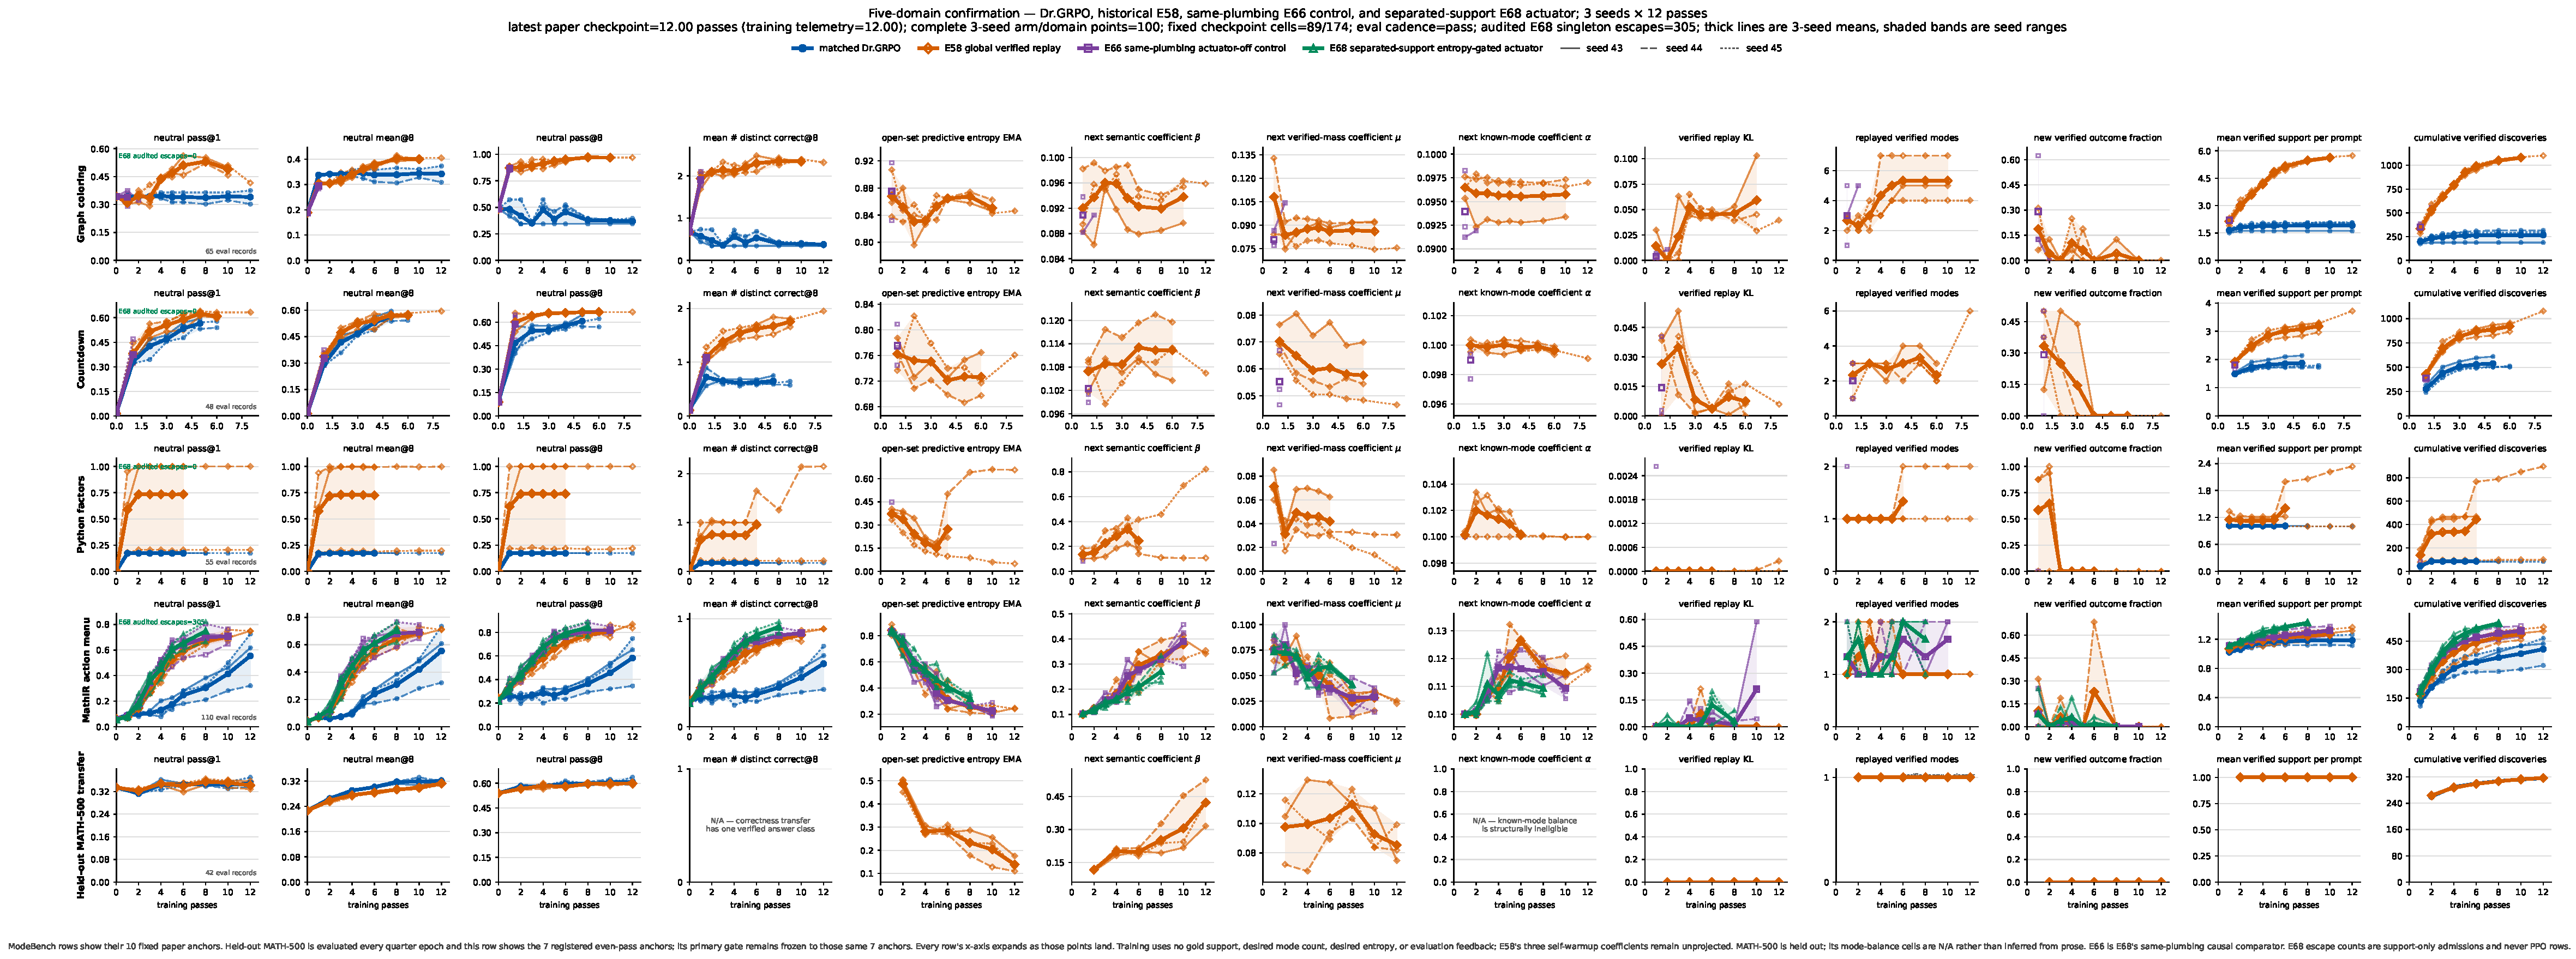
\includegraphics[width=\textheight]
    {figures/e61r1_e58_vs_grpo_05b_12ep_live.pdf}
  \caption{\textbf{The live five-domain confirmation surface.} Rows are the
  four ModeBench domains and the held-out MATH-500 transfer track; columns are
  the registered evaluation metrics followed by mechanism telemetry
  (open-set predictive entropy, the three unprojected coefficients, replay
  activity, verified support, and cumulative discoveries). Thick lines are
  three-seed means and shaded bands are seed ranges; axes expand only as fixed
  checkpoints land. MATH-500 mode-balance cells are structurally N/A rather
  than inferred from prose. This figure is regenerated from the live campaign
  artifacts and is interim.}
  \label{fig:five-domain}
\end{sidewaysfigure}

Every value in this section is read from one live snapshot, generated
\texttt{2026-07-27T22:48Z}, of a campaign that is still executing; the surface
grows monotonically as checkpoints land, so a later regeneration will show
more coverage rather than different history. At that snapshot the campaign
audit is \texttt{in\_progress}: 7 of 54 registered runs are terminal, 79 of
174 fixed arm/domain checkpoint cells and 936 of 2,046 required seed-metric
values have landed, and the integrity, cadence, equivalence, and separation
audits report zero violations. The evaluation-cadence audit passes over all 44
progressed runs. Every interpretation gate is \texttt{pending}.

\subsection{Verified MaxEnt versus matched Dr.GRPO}

Table~\ref{tab:interim} reports the latest registered checkpoint that all
three seeds of both arms have landed in each domain. The direction is
consistent across four structurally different validators, and the separation
is concentrated in breadth rather than in per-draw accuracy. Graph coloring is
the most advanced and the most separated: at pass 10 the reward-only policy
has concentrated to the point where \texttt{pass@8} (.372) is essentially its
greedy accuracy (.344) and excess multiplicity is .021, while the treatment
reaches .968 \texttt{pass@8}, 2.344 distinct correct modes, and excess
multiplicity 1.376. Countdown at pass 5 shows a small \texttt{pass@8} gain
(+.057) alongside a large breadth gain (+1.024 distinct modes).

Python factors separate on both axes but with the widest seed dispersion in
the campaign: at pass 6 the control is pinned at .172 on every metric and
every seed, while treatment seeds 43 and 44 reach 1.000 \texttt{pass@8} and
seed 45 reaches .219. The three-seed mean of .740 should not be read without
that range. MathIR action menus at pass 5 show the treatment more than
doubling both \texttt{pass@8} (.266 to .663) and greedy accuracy (.174 to
.529), the one domain where the breadth gain is accompanied by a comparable
gain in per-draw correctness.

\begin{table}[H]
  \centering
  \small
  \setlength{\tabcolsep}{4.2pt}
  \begin{tabular}{@{}llcccccc@{}}
    \toprule
    \textbf{Domain} & \textbf{Method} & \textbf{pass} & \texttt{pass@8} &
    \texttt{mean@8} & \texttt{distinct@8} & \texttt{excess} &
    \texttt{pass@1} \\
    \midrule
    Graph coloring & Dr.GRPO & 10 &
    .372 & .344 & .393 & .021 & .344 \\
    & verified MaxEnt & 10 &
    \textbf{.968} & \textbf{.400} & \textbf{2.344} & \textbf{1.376} &
    \textbf{.490} \\
    & paired mean change & &
    \(+.595\) & \(+.056\) & \(+1.951\) & \(+1.355\) & \(+.146\) \\
    \midrule
    Countdown & Dr.GRPO & 5 &
    .608 & .566 & .650 & .042 & .565 \\
    & verified MaxEnt & 5 &
    \textbf{.665} & \textbf{.571} & \textbf{1.674} & \textbf{1.010} &
    \textbf{.625} \\
    & paired mean change & &
    \(+.057\) & \(+.005\) & \(+1.024\) & \(+.967\) & \(+.060\) \\
    \midrule
    Python factors & Dr.GRPO & 6 &
    .172 & .172 & .172 & .000 & .172 \\
    & verified MaxEnt & 6 &
    \textbf{.740} & \textbf{.725} & \textbf{.956} & \textbf{.216} &
    \textbf{.734} \\
    & paired mean change & &
    \(+.568\) & \(+.553\) & \(+.784\) & \(+.216\) & \(+.563\) \\
    \midrule
    MathIR action menu & Dr.GRPO & 5 &
    .266 & .179 & .266 & .000 & .174 \\
    & verified MaxEnt & 5 &
    \textbf{.663} & \textbf{.491} & \textbf{.682} & \textbf{.019} &
    \textbf{.529} \\
    & paired mean change & &
    \(+.397\) & \(+.312\) & \(+.416\) & \(+.019\) & \(+.354\) \\
    \bottomrule
  \end{tabular}
  \caption{\textbf{Interim three-seed means at the latest shared registered
  checkpoint.} Excess multiplicity is
  \(\texttt{distinct@8}-\texttt{pass@8}\). Domains stand at different passes
  and are not pooled. Training continues toward the fixed 12-pass endpoint;
  none of these values is terminal and none evaluates a gate. Per-seed values
  are in Appendix~\ref{app:per-seed}.}
  \label{tab:interim}
\end{table}

\subsection{The actuator against its same-plumbing control}

Only MathIR has landed a shared three-seed checkpoint for both prospective
arms. At pass 5 the separated-support actuator sits .021 below the
actuator-off control on \texttt{pass@8} (.742 versus .762) and .006 above it
on \texttt{distinct@8} (.791 versus .785). A post-specified crossed bootstrap
over the three paired seeds and the shared evaluation prompts gives
descriptive 95\% intervals of \([-.095,.052]\) for \texttt{pass@8} and
\([-.074,.085]\) for \texttt{distinct@8}: the paired seed deltas disagree in
sign in both cases. This analysis was frozen before integration, computes no
\(p\)-values, and cannot change any gate; it also does not turn three training
seeds into more than three independent runs. Python factors, where the repair
hypothesis is actually directed, has no landed comparison yet.

The mechanism telemetry is more informative than these early performance
deltas, because it is what makes the repair falsifiable. The controller must
first detect an entropy deficit, and the actuator must then intervene cleanly.
Both halves are visible. In Python, the treatment's open-set entropy EMA has
fallen well below each run's own warmup reference for two of three seeds
(ratios .431 and .122 against .951 for the third), and the unprojected
coefficient has risen correspondingly (.220 and .822 against .105) with no
projection ever active; the collapsed seed sits at mean bank support exactly
1.000, which is precisely the singleton state the actuator targets. The
separated-support arm has recorded 286 audited entropy-gated interventions
over 6,550 metric-bearing updates (4.37 per 100), all in MathIR, with a
maximum of one alternate admitted in any proposal group, zero proposal rows
sent to PPO, and zero objective-count overlaps across 118 audited
proposal-only outcomes and 157 outcomes that later graduated to neutral
on-policy discoveries. The domains with no interventions have no
metric-bearing updates yet; zero interventions is the expected reading before
a registered collapse condition occurs, and the terminal gate cannot pass
without at least one clean intervention.

\subsection{Held-out MATH-500 transfer}

\begin{figure}[H]
  \centering
  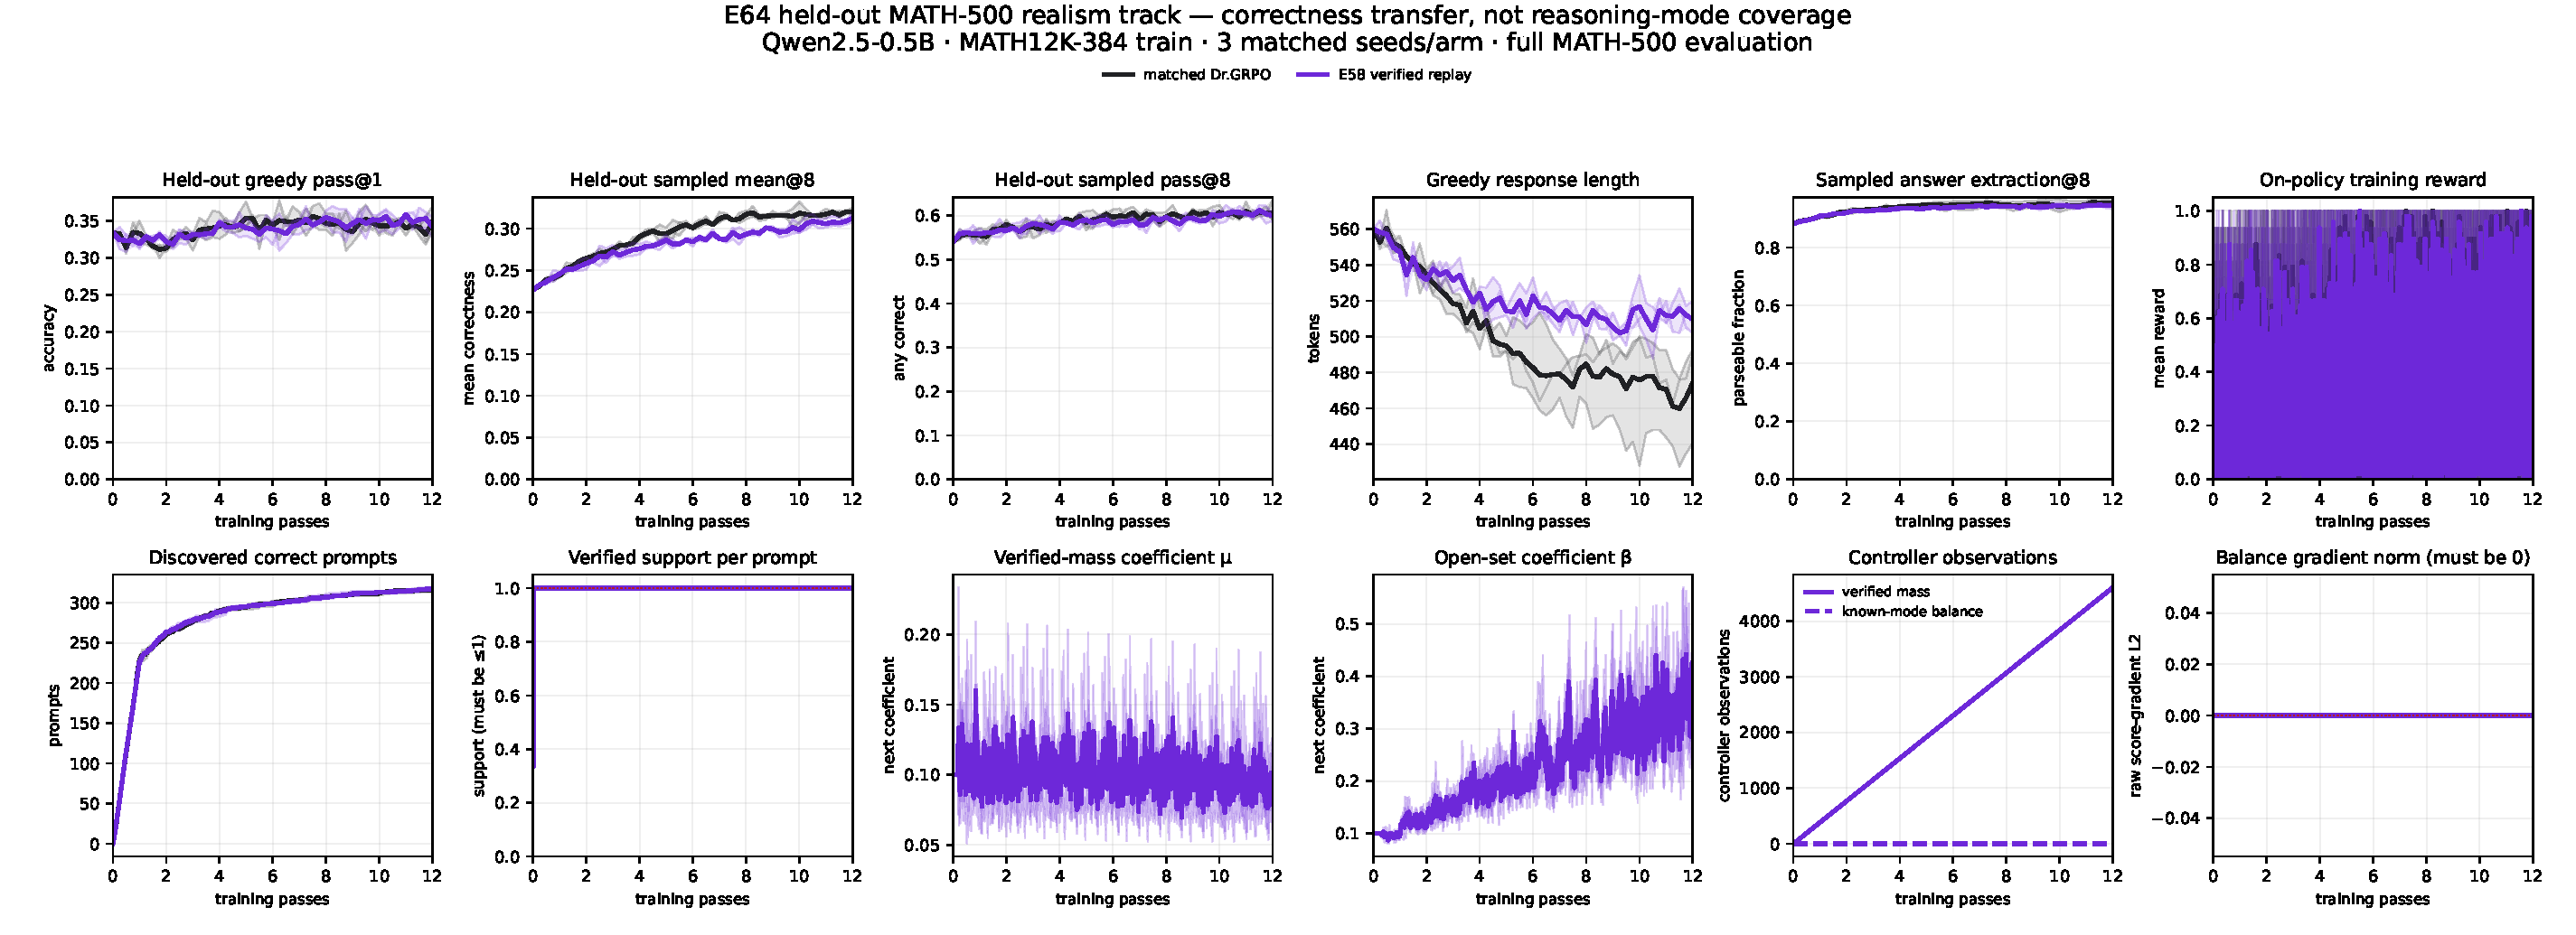
\includegraphics[width=\linewidth]
    {figures/e64_math500_realism_05b_12ep_live.pdf}
  \caption{\textbf{Held-out MATH-500 realism track.} Correctness transfer
  after training on 384 frozen MATH12K rows, evaluated on all 500 held-out
  problems. The bottom row confirms the structural contract: verified support
  per prompt never exceeds one, the balance gradient is identically zero, and
  the mass and open-set coefficients remain finite and unprojected. Interim;
  the registered anchors run to pass 12.}
  \label{fig:math500}
\end{figure}

At pass 2 the two arms are close on every held-out metric: greedy
\texttt{pass@1} .322 versus .313 for the control, \texttt{mean@8} .258 versus
.265, and \texttt{pass@8} .566 versus .579. The treatment is directionally
higher on greedy accuracy and slightly lower on the sampled metrics, and all
three gaps are smaller than the seed-to-seed spread within either arm. The
registered gate needs terminal values at pass 12 and a \(.02\) non-inferiority
margin, so nothing here decides it. The structural contract does hold as
registered: verified support per prompt stays at one, known-mode balance
contributes exactly zero gradient, and both active coefficients remain finite
and unprojected. A supplemental verifier-sensitivity audit is
\texttt{in\_progress}, with 93 caught timeout diagnostics and zero
identical-response reward conflicts.

\subsection{What is not yet a result}

No terminal comparison exists in any domain. Seven of 54 runs have reached
pass 12, and Graph coloring's Dr.GRPO arm is the only complete registered
trajectory. No AUC is emitted, because partial AUC over an incomplete
checkpoint set cannot pass a gate. The actuator's target domain has no landed
comparison, the plumbing-sensitivity contrast has only partial coverage, and
the transfer gate is six checkpoints short. Every value in this section is a
progress reading against a frozen surface, and a \texttt{pending} gate is
evidence of neither success nor failure.

\section{How the Development Evidence Determines the Final Design}
\label{sec:design-history}

The final method is easier to understand as a sequence of ruled-out
alternatives. We report those decisions because they constrain what the
current evidence means, not because every exploratory run is an independent
experiment.

Finite-action studies supplied the positive reference point. When every
semantic answer was represented by a fixed short action and the full action
distribution could be enumerated, direct complete-action MaxEnt preserved
substantially more breadth than reward-only training. That result established
that the entropy mechanism can work when representation and measurement are
aligned. It did not solve the present problem: the codec changes the policy,
requires a task-specific action set, and may expose a gold-derived support.
The online bank retains the executable semantic object while learning support
only from policy demonstrations.

Reward-based candidate aggregation provided a second useful boundary. It can
focus learning on the successful members of a mixed group, but it remains
uniform in an all-equal or all-wrong group and cannot create a missing outcome.
Conversely, a semantic term can preserve rare verified outcomes but becomes
sparse when successes disappear. The final objective therefore keeps task
advantage and canonical discovery on separate channels rather than asking
either to substitute for the other.

\begin{table}[H]
  \centering
  \small
  \begin{tabularx}{\linewidth}{@{}YYY@{}}
    \toprule
    \textbf{Observed failure} & \textbf{Why it matters} &
    \textbf{Decision retained here} \\
    \midrule
    Sequence entropy increased length and EOS avoidance &
    Token uncertainty can grow without solution breadth &
    Measure and optimize validator-bound outcomes \\
    Candidate-local normalization favored short samples &
    A nominally uniform target can create a nonzero length gradient &
    Keep canonical pressure as a separate detached advantage \\
    Detached candidate fitting optimized the wrong population target &
    Reweighting samples is not the same as policy MaxEnt &
    State the empirical outcome objective precisely \\
    Group-centered surprise vanished as samples concentrated &
    A controller cannot amplify a carrier with zero dispersion &
    Center under the predictive bank distribution, outside task centering \\
    Novel wrong answers received diversity pressure &
    Error variety is not useful solution diversity &
    Admit and reward only validator-positive outcomes \\
    Fixed pressure weakened after support growth and late collapse &
    Raw entropy has a moving maximum &
    Normalize the sensor and reference it to the run's own warmup \\
    A bounded controller saturated below its target &
    The ceiling, not the target, became the active intervention &
    Remove every projection and report coefficient growth \\
    Prompt-local replay left late singletons idle for nearly a pass &
    A discovery that cannot act promptly is not an actuator &
    Schedule one verified bank globally on every update \\
    A singleton bank made every diversity term ineligible &
    The mechanism is unidentifiable exactly where collapse is worst &
    Add a support-only escape gated on the run's own entropy deficit \\
    A shared proposal/on-policy bank leaked off-policy support &
    Proposed outcomes would enter an on-policy advantage &
    Separate proposal support from the objective count table \\
    \bottomrule
  \end{tabularx}
  \caption{\textbf{Decision provenance.} Earlier work is used as design
  evidence. The paper does not pool superseded objectives into the final
  treatment estimate.}
  \label{tab:decisions}
\end{table}

This history also explains why ordinary final-answer mathematics appears only
as a transfer track. A correct boxed number does not prove that a claimed
intermediate strategy was executed. Restricted algebra programs demonstrated
that executable strategy keys are possible. Repeated calibration of heuristic
strategy labelers, finite menus, and cross-checked natural-language routes
exposed false merges, false distinctions, and plausible but invalid
derivations; adding more judges did not turn labels into execution. The MathIR
action menu is what survived that program: the menu is finite, the
transformations execute under exact rational arithmetic, and the key comes
from the resulting state trajectory. MATH-500 is retained only as a
correctness-transfer test, with mode language explicitly forbidden.

\section{Discussion}
\label{sec:discussion}

\paragraph{A benchmark about discovery, not catalogues.}
Exact valid-mode counts make coverage interpretable at evaluation time, but
training never receives a list of valid answers. The bank contains only what
the current policy has demonstrated. This separates the scientific question
``does the policy discover and retain alternatives?'' from the easier problem
of regularizing toward a supplied menu.

\paragraph{Why an open-set predictor is necessary but imperfect.}
The structural unseen bucket keeps the sensor honest about undiscovered
support and makes a two-mode prompt and a ten-mode prompt comparable relative
to what has been observed. It still does not estimate entropy over
undiscovered modes, and cumulative counts make it a slow, history-dependent
sensor. The discovery credit is therefore not redundant: it pays for expanding
support, while the predictive term balances the support already observed.

\paragraph{Why projection-free coefficients are a scientific stress test.}
Removing every bound is not a claim that unbounded pressure is always safe. It
makes saturation observable. If the sensor stays below its own reference, the
coefficient can grow until the policy responds or quality fails, and the
interim Python telemetry shows exactly that regime: a coefficient at .822
while mean bank support sits at 1.000. The 12-pass design must report both
outcomes, and a successful treatment needs breadth without runaway invalidity
or loss of per-sample correctness.

\paragraph{Why the actuator needed its own control.}
Enabling counterfactual proposals also changed the sampling and weight-sync
path. Comparing the actuator against the historical treatment would have
confounded the mechanism with its plumbing, so the campaign spends twelve runs
on an actuator-off arm that shares the new execution surface exactly. The
same discipline forced the separation contract: an earlier design was rejected
before optimization because one shared bank would have let proposed support
change the next on-policy advantage.

\paragraph{Executable domains strengthen the semantic claim.}
Graph assignments and expression ASTs could be dismissed as bespoke
canonicalizers. Python factors use the same abstract contract but a different
implementation boundary: syntax is screened, a separate interpreter makes
several calls, and the resulting behavior vector defines the mode. MathIR adds
a fourth boundary in which the mode is a procedure rather than an answer. Two
different source strings that behave identically collapse to one key; one
source string that returns a different valid vector occupies another mode.

\section{Limitations and Broader Impact}
\label{sec:limitations}

The main empirical limitation is incompleteness. Seven of 54 registered runs
are terminal, no gate has been evaluated, and the actuator's target domain has
no landed comparison. The reported snapshot is frozen, paired, and honest
about which checkpoint each domain stands at, but it is a progress reading.
Three seeds describe paired directions rather than a population distribution,
and the method was selected after an extensive outcome-informed development
program, so all claims are exploratory. The campaign has also required several
placement amendments after preemptions, GPU drains, and one contaminated
allocation; these are hash-bound and change placement only, but they are part
of the provenance.

All tasks are synthetic, the trained model has 0.5B parameters, and exact
mode identity is unusually available. Mode coverage in open-ended reasoning
may be unknowable. A canonicalizer can also merge solutions that matter or
split aliases that do not. We mitigate that risk by deriving keys from
execution, documenting equivalences, and refusing to label free-form proof
strategies without an adequate validator.

Executing generated code is hazardous. The Python environment admits only a
small call-free AST, removes builtins, runs outside the trainer process, bounds
the input domain, enforces a timeout, and fails closed. It is a program
behavior benchmark, not a general sandbox for arbitrary model code.

The work does not directly increase deployment capability. Its benefit is
methodological: it makes diversity claims auditable and separates sampled
breadth from average correctness. The same machinery could overvalue novelty
when a task's valid modes are not equally useful. Applications should report
quality, breadth, invalidity, and the mode mapping together.

\section{Conclusion}
\label{sec:conclusion}

Solution diversity is not token entropy and not the number of different
strings a model can emit. \textsc{ModeBench} treats it as a validator-bound
execution outcome. Online verified MaxEnt then learns only from correct modes
the policy has demonstrated, rewards first discovery separately from
frequency balancing, replays discovered banks promptly through a global
schedule, and adapts every coefficient against the run's own history rather
than an external target.

The confirmatory campaign is unfinished, but its interim fixed-checkpoint
surface already shows the intended separation on four structurally different
executable validators: much higher sampled breadth, with per-draw accuracy
that is preserved on graph coloring and Countdown and improved on Python
factors and MathIR. Held-out MATH-500 transfer is currently within a point of
the matched control in both directions. Terminal pass-12 values across all 54
registered runs, and the four frozen gates they will decide, remain the next
evidence required.

\bibliographystyle{plainnat}
\bibliography{example_paper}

\appendix
\onecolumn

\section{External Python Verification Contract}
\label{app:python}

The Python response is parsed in expression mode and must have an AST rooted
at a lambda with exactly one argument named \(n\). The accepted node set is:
lambda arguments, integer constants, \(n\), arithmetic operators
\(\{+,-,\times,//,\bmod\}\), comparisons, Boolean operators, unary
\(+,-,\mathrm{not}\), and conditional expressions. The parser rejects calls,
attributes, imports, comprehensions, collections, subscripts, assignment,
loops, and every other identifier. Candidate length and AST node count are
bounded.

The parent process sends the restricted source and trusted JSON task
specification to a persistent isolated interpreter over JSON lines. The worker
re-parses the source, removes builtins, evaluates the lambda, and invokes it on
the frozen inputs under a per-request timer. It returns only validity, the
integer output vector, and the canonical key. A timeout, broken pipe, malformed
response, non-integer value, or divisor failure yields no key. The parent can
restart a failed worker.

For example, with inputs \([6,10,15]\),
\[
\texttt{lambda n: 2 if n \% 2 == 0 else 3}
\]
returns \((2,2,3)\), while
\[
\texttt{lambda n: 3 if n \% 3 == 0 else 5}
\]
returns \((3,5,3)\). Both verify and receive different keys. The repository
audit command is:

\begin{verbatim}
python ops/verify_python_factor_mode.py \
  --candidate 'lambda n: 2 if n % 2 == 0 else 3' \
  --reference \
  '{"verifier":"python_factor_function",
    "python_version":"factor-v1","cases":[6,10,15]}'
\end{verbatim}

\section{Dataset Audits}
\label{app:python-data}

The deterministic Python materialization uses seed 5100, four tool calls per
prompt, and composite inputs at most 96. The MathIR action-menu
materialization uses seed 5900, four equation families, at most eight menu
actions, and at most four program steps, with the exhaustive mode set
enumerated per family and withheld from training. Their identities are:

\begin{center}
\begin{tabular}{@{}lrr@{}}
\toprule
& \textbf{Python factors} & \textbf{MathIR action menu} \\
\midrule
Training rows & 384 & 384 \\
Evaluation rows & 128 & 128 \\
Exact modes per prompt & 16--3,600 & 5 \\
Training-row SHA-256 &
\texttt{bcfa9acc\ldots37cf7} & \texttt{bfc98362\ldots5d3835} \\
Evaluation-row SHA-256 &
\texttt{be0f621c\ldots94d183} & \texttt{df5783dd\ldots328b96} \\
Gold catalogue supplied to policy & no & no \\
Training bank initialization & empty & empty \\
\bottomrule
\end{tabular}
\end{center}

For every Python row, the generator selects the smallest and largest proper
divisor for each input, writes two nested-conditional lambda programs, and
sends both to the external worker. Materialization aborts unless both verify
and return different keys. The exact mode count is computed independently as
the product of divisor-set sizes. Train and evaluation input tuples are
disjoint. For every MathIR family, the certified routes are executed and
canonicalized through the same interpreter that scores model responses.

\section{Per-Seed Interim Endpoints}
\label{app:per-seed}

\begin{table}[H]
  \centering
  \small
  \begin{tabular}{@{}llrcccc@{}}
    \toprule
    \textbf{Domain (pass)} & \textbf{Method} & \textbf{Seed} &
    \texttt{pass@8} & \texttt{mean@8} & \texttt{distinct@8} &
    \texttt{pass@1} \\
    \midrule
    Graph (10) & Dr.GRPO & 43 & .344 & .344 & .344 & .344 \\
    & & 44 & .388 & .327 & .409 & .323 \\
    & & 45 & .385 & .361 & .427 & .365 \\
    & verified MaxEnt & 43 & .971 & .396 & 2.336 & .500 \\
    & & 44 & .964 & .397 & 2.302 & .458 \\
    & & 45 & .969 & .406 & 2.393 & .510 \\
    \midrule
    Countdown (5) & Dr.GRPO & 43 & .648 & .594 & .750 & .594 \\
    & & 44 & .572 & .537 & .588 & .531 \\
    & & 45 & .604 & .565 & .613 & .570 \\
    & verified MaxEnt & 43 & .664 & .559 & 1.846 & .609 \\
    & & 44 & .672 & .576 & 1.521 & .625 \\
    & & 45 & .658 & .577 & 1.656 & .641 \\
    \midrule
    Python (6) & Dr.GRPO & 43 & .172 & .172 & .172 & .172 \\
    & & 44 & .172 & .172 & .172 & .172 \\
    & & 45 & .172 & .172 & .172 & .172 \\
    & verified MaxEnt & 43 & 1.000 & .995 & 1.000 & 1.000 \\
    & & 44 & 1.000 & .993 & 1.648 & 1.000 \\
    & & 45 & .219 & .188 & .219 & .203 \\
    \midrule
    MathIR (5) & Dr.GRPO & 43 & .318 & .221 & .318 & .227 \\
    & & 44 & .244 & .167 & .244 & .164 \\
    & & 45 & .236 & .148 & .236 & .133 \\
    & verified MaxEnt & 43 & .727 & .553 & .752 & .586 \\
    & & 44 & .590 & .430 & .607 & .477 \\
    & & 45 & .674 & .489 & .688 & .523 \\
    \midrule
    MathIR (5) & actuator-off control & 43 & .811 & .613 & .828 & .656 \\
    & & 44 & .676 & .436 & .709 & .469 \\
    & & 45 & .801 & .646 & .818 & .680 \\
    & separated-support actuator & 43 & .729 & .574 & .770 & .617 \\
    & & 44 & .703 & .497 & .750 & .555 \\
    & & 45 & .793 & .572 & .854 & .641 \\
    \midrule
    MATH-500 (2) & Dr.GRPO & 43 & .578 & .262 & --- & .316 \\
    & & 44 & .590 & .266 & --- & .308 \\
    & & 45 & .570 & .266 & --- & .316 \\
    & verified MaxEnt & 43 & .572 & .265 & --- & .322 \\
    & & 44 & .562 & .251 & --- & .314 \\
    & & 45 & .564 & .259 & --- & .330 \\
    \bottomrule
  \end{tabular}
  \caption{\textbf{Seed-level values underlying Table~\ref{tab:interim} and
  Section~\ref{sec:results}.} Each block is at the latest registered
  checkpoint landed by all three seeds of both compared arms.
  \texttt{distinct@8} is omitted for MATH-500 because a single-answer task has
  no reasoning-mode surface.}
  \label{tab:per-seed}
\end{table}

\section{Supplemental All-Epoch Diagnostic}
\label{app:diagnostic}

\begin{sidewaysfigure}
  \centering
  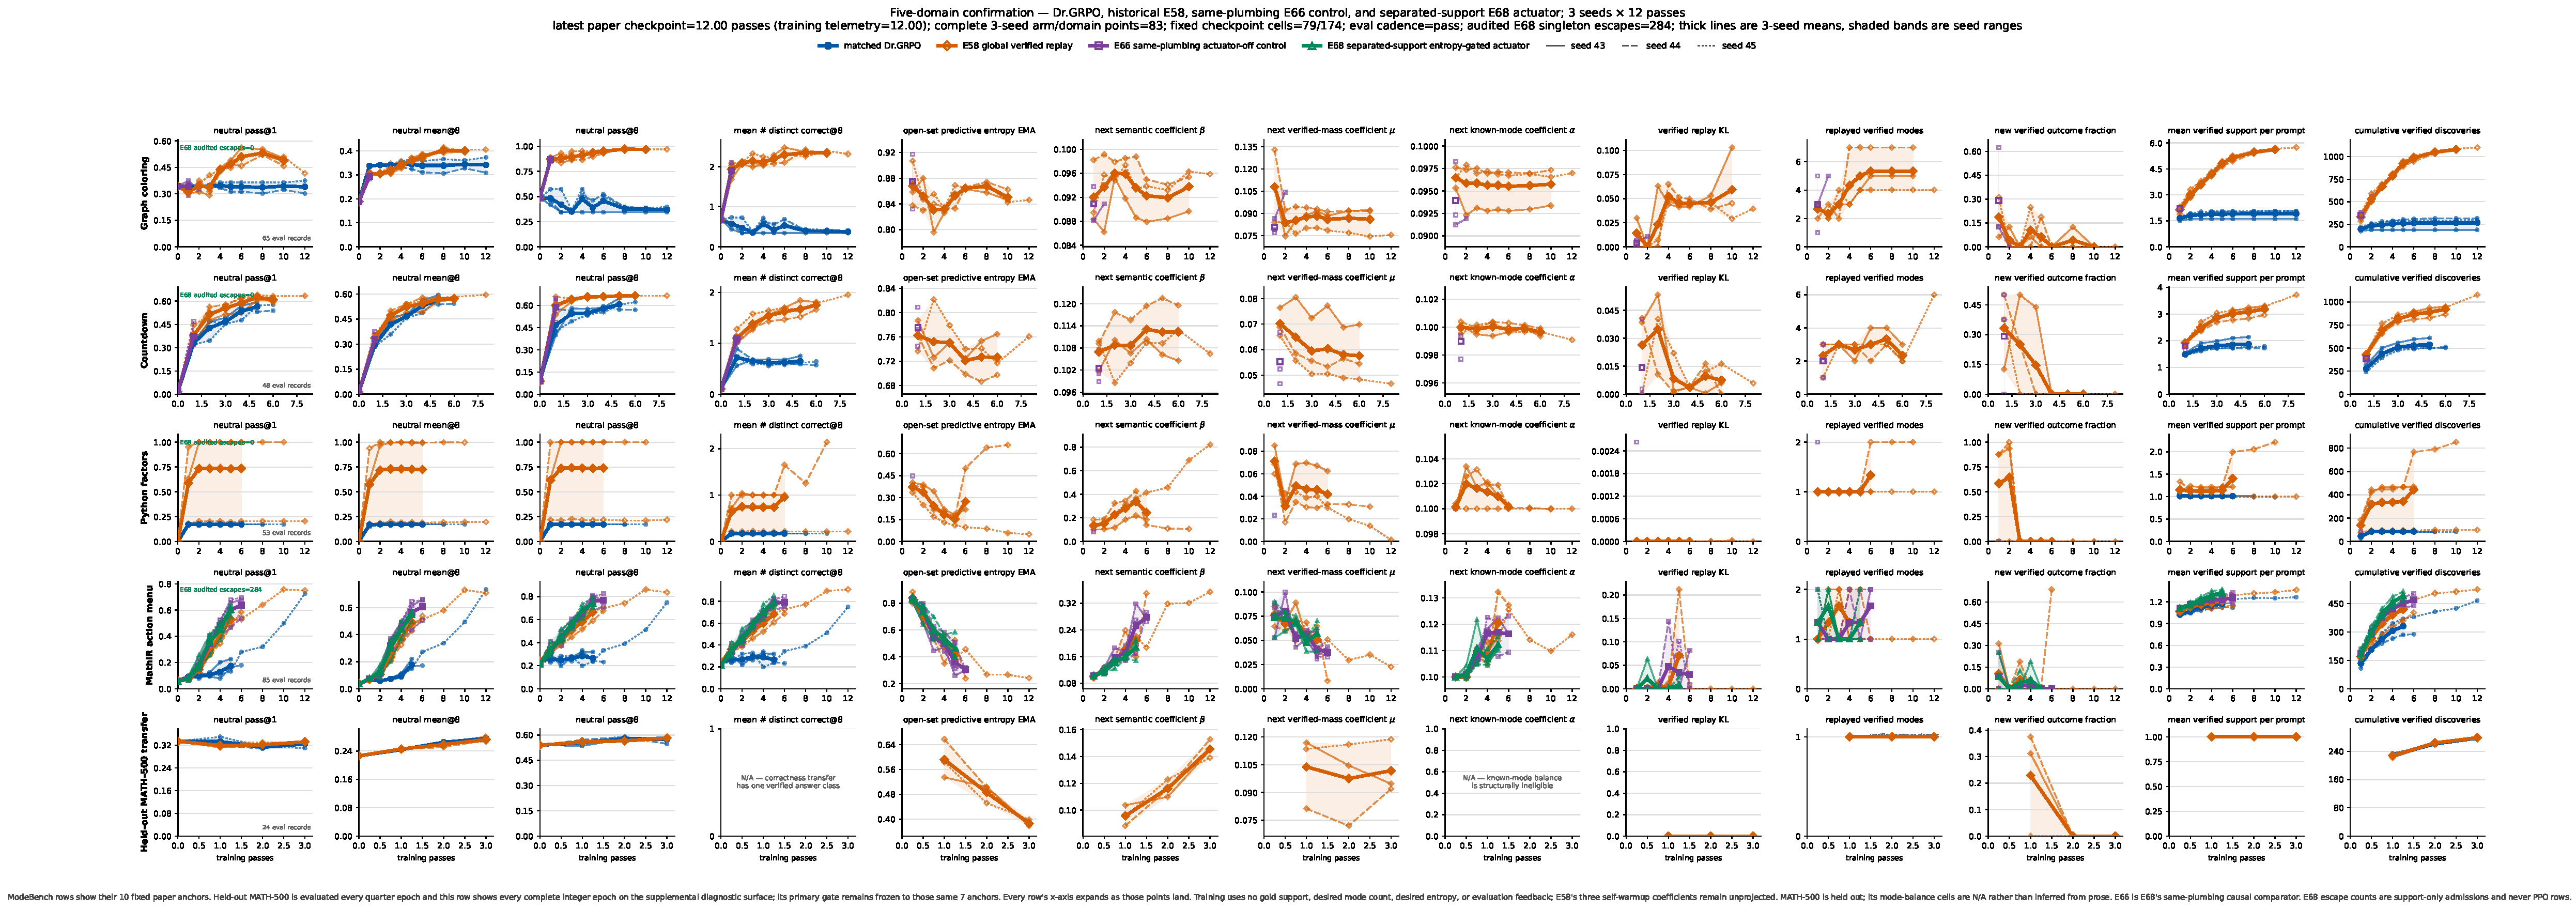
\includegraphics[width=\textheight]
    {figures/e61r1_e58_vs_grpo_05b_12ep_all_epoch_diagnostic_live.pdf}
  \caption{\textbf{Every complete integer epoch.} This diagnostic overrides
  only the MATH-500 display surface, expanding it from the seven registered
  even-pass anchors to all thirteen integer epochs already present in the
  retained quarter-epoch traces. It exists so that monitoring can stay
  granular without silently changing the estimand: the primary figure, tables,
  and realism gate remain frozen to the registered anchors.}
  \label{fig:diagnostic}
\end{sidewaysfigure}

\section{Reproducibility and Evidence Boundaries}
\label{app:reproducibility}

The live confirmation surface is regenerated on a fixed interval by
\path{ops/exp_scaling/watch_e65_entropy_gated_singleton_confirmation.sh},
which runs the audit chain, reparses every curve, rewrites
\path{paper/results/e65_five_domain_confirmation_live.md} and its seed-level
CSV, and re-renders both figures in this paper. The machine-readable surface
is \path{var/artifacts/e65_five_domain_confirmation_results_latest.json}, and
the final claim gate is
\path{ops/exp_scaling/audit_e65_legitimate_result_readiness.py}, which cannot
report success while any registered run, checkpoint cell, cadence
requirement, or interpretation gate is outstanding.

The four ModeBench environments are implemented in
\path{src/oat_drgrpo/canonical_actions.py},
\path{src/oat_drgrpo/python_modebench.py}, and
\path{src/oat_drgrpo/mathir.py}; the external Python process boundary and
worker are in \path{src/oat_drgrpo/python_modebench_process.py} and
\path{src/oat_drgrpo/python_modebench_worker.py}. The open-set predictive
signal and its controller are in \path{src/oat_drgrpo/semantic_shannon.py},
the split replay objective in \path{src/oat_drgrpo/canonical_replay.py}, the
bank in \path{src/oat_drgrpo/online_canonical_bank.py}, and the singleton
actuator in \path{src/oat_drgrpo/counterfactual_proposals.py}. Deterministic
generators are \path{ops/make_python_factor_mode_data.py} and
\path{ops/make_mathir_action_menu_data.py}. Every protocol and every
placement amendment cited in Section~\ref{sec:experiments} is a frozen
document under \path{paper/preregistration/}.

The manuscript deliberately separates four evidence classes:

\begin{enumerate}
  \item historical engineering and mechanism evidence, used to motivate the
  final design but not pooled into its effect estimate;
  \item the 54-run registered campaign, whose incomplete fixed-checkpoint
  snapshot appears in Section~\ref{sec:results} and whose four gates remain
  \texttt{pending};
  \item benchmark audits, which establish executable multiple modes and exact
  mode counts but are not RL results; and
  \item invalidated cohorts, excluded from the campaign denominator by
  machine-readable audits and retained only as engineering evidence.
\end{enumerate}

\end{document}
